\documentclass[11pt,letterpaper]{article}
\usepackage[lmargin=1in,rmargin=1in,bmargin=1in,tmargin=1in]{geometry}
\usepackage{style/quiz}
\usepackage{style/commands}

% -------------------
% Content
% -------------------
\begin{document}
\thispagestyle{title}


% Quiz 1
\quizsol \textit{True/False}: If $P$ is the proposition $6 < 5$ and $Q$ is the proposition, ``Earth is a planet,'' then the logical statement $P \to Q$ is false. \pspace

\sol The statement is \textit{false}. Recall that the truth table for $P \to Q$ is as follows: \par
	\begin{table}[!ht]
	\centering
	\begin{tabular}{c|c|c}
	$P$ & $Q$ & $P \to Q$ \\ \hline
	$T$ & $T$ & $T$ \\
	$T$ & $F$ & $F$ \\
	$F$ & $T$ & $T$ \\
	$F$ & $F$ & $T$
	\end{tabular}
	\end{table} \par
Here, $P$ is the proposition $P: 6 < 5$ and $Q$ is the proposition $Q$: ``Earth is a planet.'' It is clear that $P$ is false and $Q$ is true. But then examining the logic table above, we can see that $P \to Q$ is true. \pvspace{1.5cm}



% Quiz 2
\quizsol \textit{True/False}: $\neg (P \to \neg Q) \equiv P \wedge Q$ \pspace

\sol The statement is \textit{true}. To determine if two propositions are logically equivalent, one can either examine the truth table or apply logical rules to obtain one logical expression from the other. If we construct a truth table, we have\dots \par
	\begin{table}[!ht]
	\centering
	\begin{tabular}{c|c||c|c|c||c}
	$P$ & $Q$ & $\neg Q$ & $P \to \neg Q$ & $\neg (P \to \neg Q)$ & $P \wedge Q$ \\ \hline
	$T$ & $T$ & $F$ & $F$ & $T$ & $T$ \\
	$T$ & $F$ & $T$ & $T$ & $F$ & $F$ \\
	$F$ & $T$ & $F$ & $T$ & $F$ & $F$ \\
	$F$ & $F$ & $T$ & $T$ & $F$ & $F$
	\end{tabular}
	\end{table}
Because for each possible pair of choices for $P$ and $Q$ the outputs for $\neg (P \to \neg Q)$ and $P \wedge Q$ match, $\neg (P \to \neg Q) \equiv P \wedge Q$. Alternatively, we can transform one into the other by applying logical equivalences (recall $P \to Q \equiv \neg P \vee Q$ or $\neg (P \to Q) \equiv P \wedge \neg Q$):
	\[
	\neg (P \to \neg Q) \equiv \neg (\neg P \vee \neg Q) \equiv \neg (\neg P) \wedge \neg (\neg Q) \equiv P \wedge Q.
	\] 




 \pvspace{0.5cm}

% Quiz 3
\quizsol \textit{True/False}: The logic corresponding to the circuit shown below is the proposition:
	\[
	(\neg P \wedge Q) \vee \neg Q.
	\]
	\begin{figure}[!ht]
	\centering
	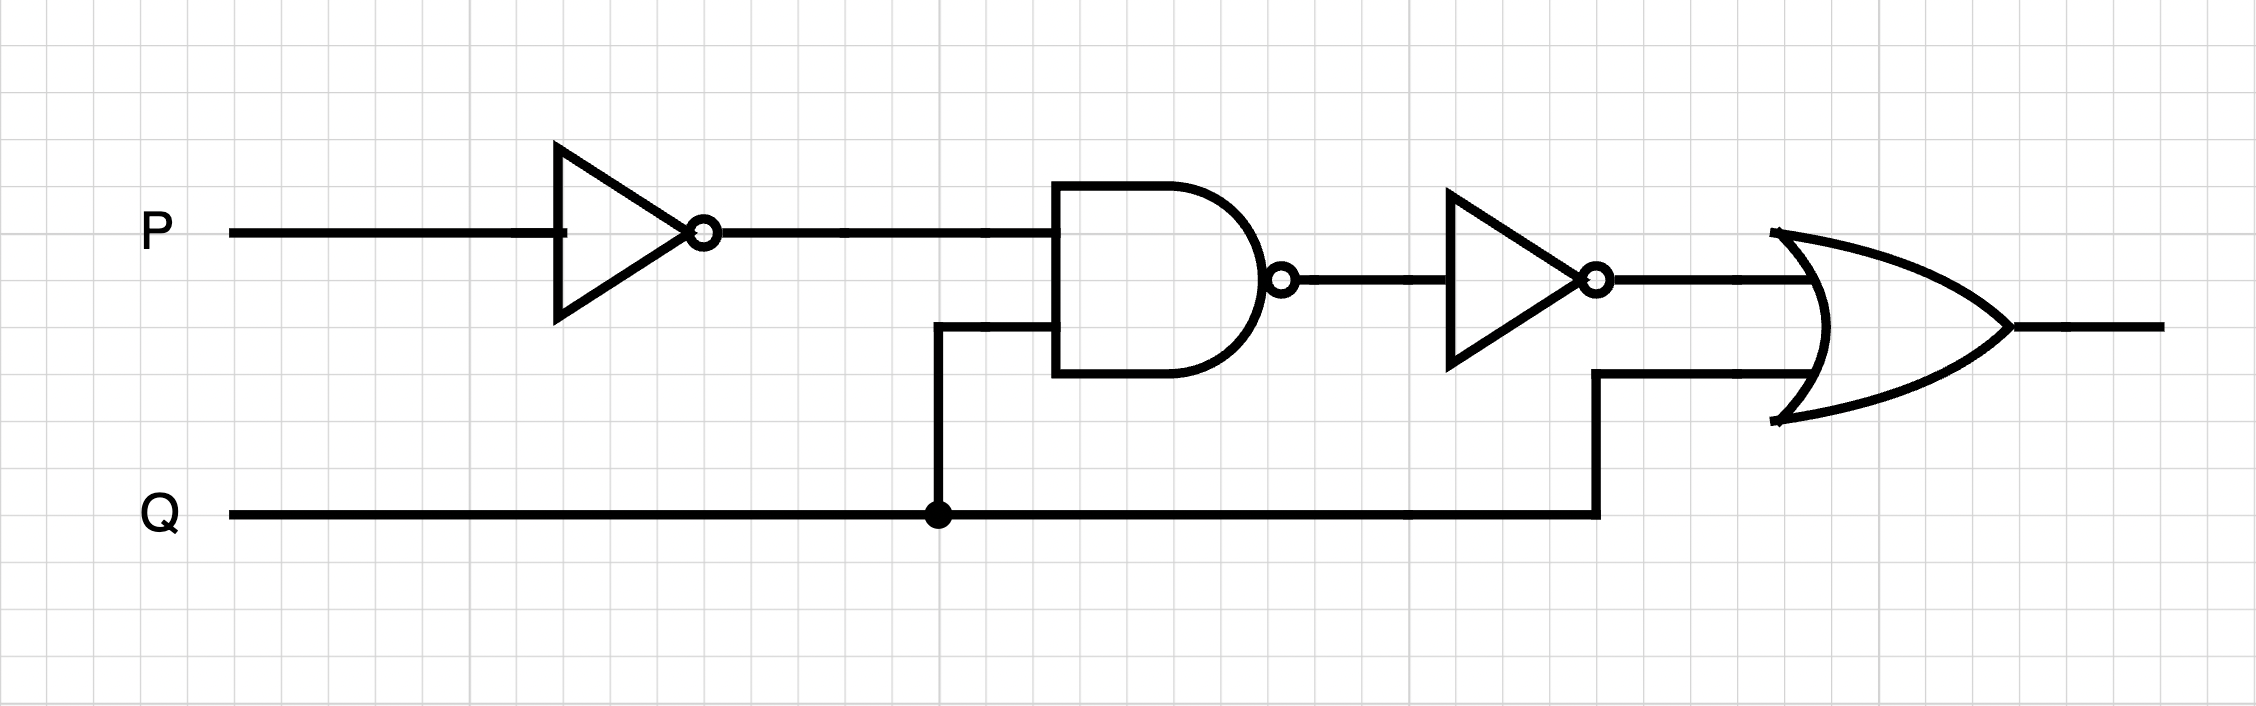
\includegraphics[width=0.74\textwidth]{images/circuit}
	\end{figure} \par

\newpage

\sol The statement is \textit{false}. We can trace through the circuit. We see that the current from $P$ passes through a NOT gate and we obtain $\neg P$. This then feeds into an AND gate along with $Q$ so that we obtain $\neg P \wedge Q$. The resulting current is then passed through a NOT gate, obtaining $\neg (\neg P \wedge Q)$. This finally reaches an OR gate---along with $Q$---to obtain $\neg (\neg P \wedge Q) \vee Q$. We can see a diagrammatic explanation below. \par
	\begin{figure}[!ht]
	\centering
	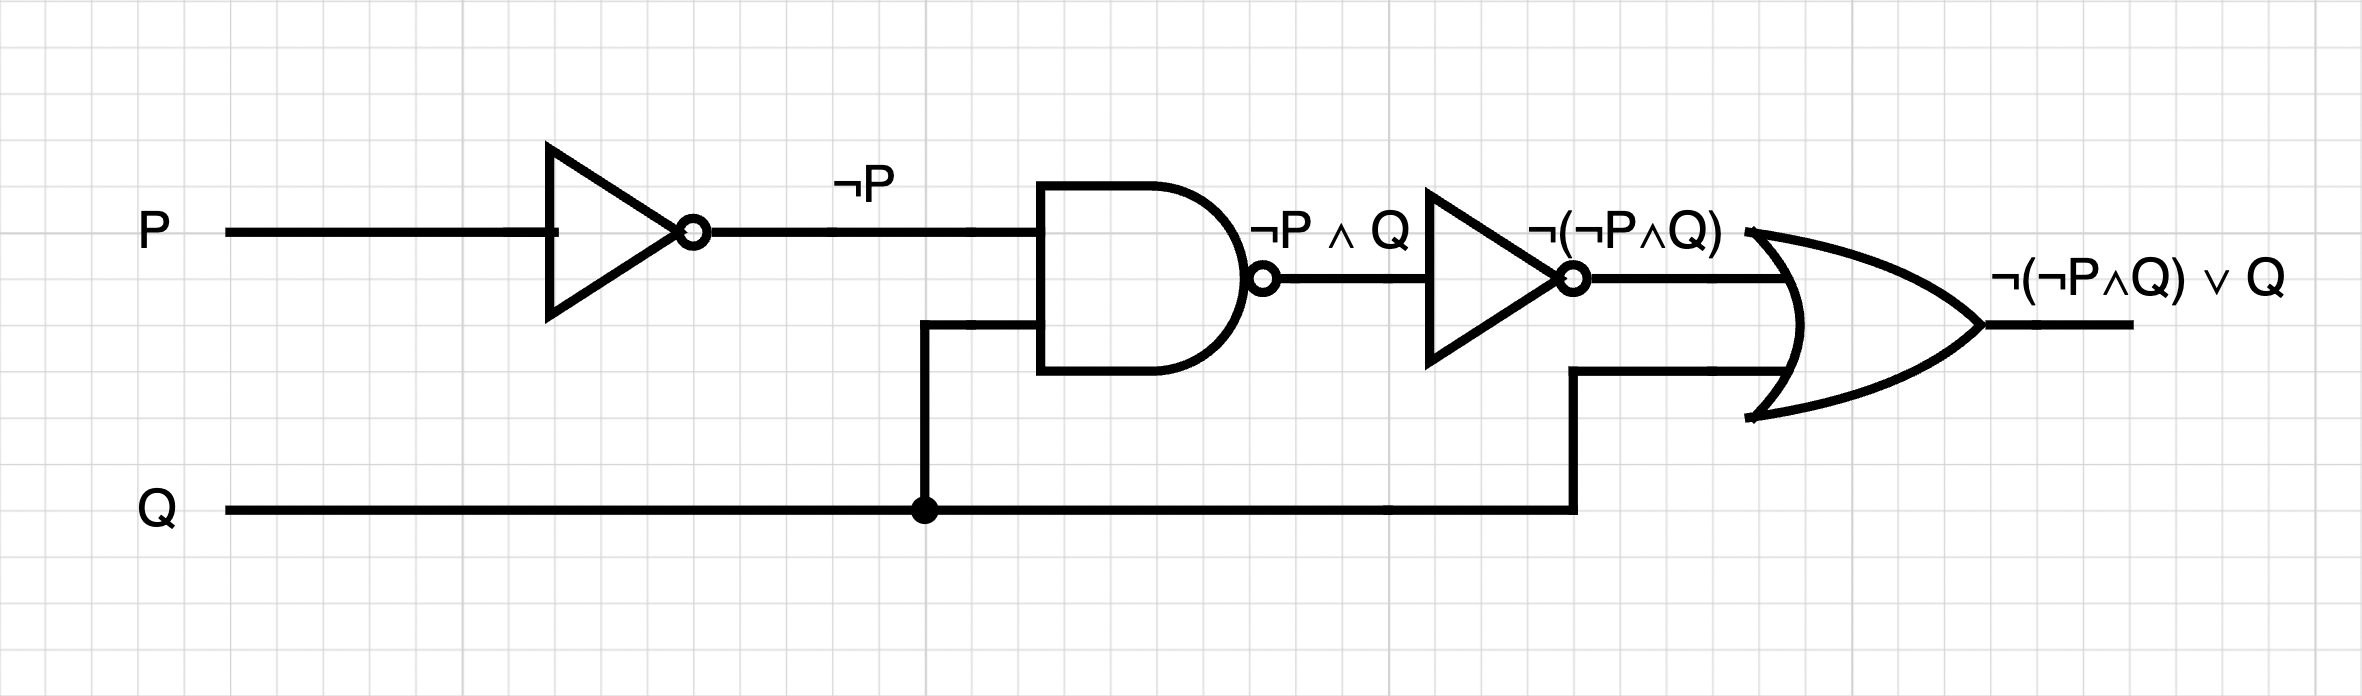
\includegraphics[width=0.74\textwidth]{images/circuit_sol}
	\end{figure} \pvspace{0.5cm}




% Quiz 4
\quizsol \textit{True/False}: Let the universe $\mathcal{U}$ be the set of real numbers and define $P(x)$ to be the predicate $P(x): x^2 + x - 4 \geq 0$. Then $(\forall x) \big(\neg P(x) \big)$ is true. \pspace

\sol The statement is \textit{false}. If $P(x): x^2 + x - 4 \geq 0$, then $\neg P(x): x^2 + x - 4 < 0$. But then $(\forall x) \big(\neg P(x) \big)$ is the statement, ``For all $x$, $x^2 + x - 4 < 0$.'' Now if $x= 1$, we have $\neg P(1) \colon 1^2 + 1 - 4 < 0$, i.e. $-2 < 0$, which is true. If $x= 0$, we have $\neg P(0) \colon 0^2 + 0 - 4 < 0$, i.e. $-4 < 0$, which is true. However, while $(\forall x) \big(\neg P(x) \big)$ is clearly true for \textit{some} (we found at least two), it is not true \textit{for all} $x$. As a counterexample, let $x= 10$. Then $\neg P(10) \colon 10^2 + 10 - 4 < 0$, which is $104 < 0$---clearly false. Therefore, $\neg P(x)$ is not true for all $x$. But then $(\forall x) \big(\neg P(x) \big)$ is false. \pvspace{1.5cm}





\end{document}